\documentclass[12pt,a4paper]{report}

% Packages
\usepackage[utf8]{inputenc}
\usepackage{setspace}
\usepackage{geometry}
\usepackage{hyperref}
\usepackage{graphicx}
\usepackage{titlesec}
\usepackage{amsmath} 
\usepackage{amssymb}
\usepackage{booktabs}
\usepackage{float}

\usepackage{tikz}
\usetikzlibrary{arrows.meta, calc, positioning, patterns, fadings}

\tikzstyle{block} = [draw, fill=white, rectangle, 
    minimum height=3em, minimum width=6em]
\tikzstyle{sum} = [draw, fill=white, circle, node distance=1cm]
\tikzstyle{input} = [coordinate]
\tikzstyle{output} = [coordinate]
\tikzstyle{pinstyle} = [pin edge={to-,thin,black}]

\onehalfspacing
\geometry{margin=1in}

\titleformat{\chapter}[hang]
  {\normalfont\huge\bfseries}
  {\thechapter.}
  {1em}
  {}

\begin{document}

\title{Applying Deep Learning on Sequential Data within the Mixed-Model Assembly Line problem}
\author{Christoffer Lindkvist}
\date{\today}
\maketitle

\begin{abstract} 
    A mixed-model assembly line manufactures different product variants on a single line, where variations in tasks can create imbalances across the workstations. When several labour-intensive models appear consecutively, some stations may exceed their capacity, leading to overloads that require halting the entire assembly line to resolve the issues. 

    This challenge is formalized as \textit{the Product Sequencing Problem}, an NP-hard optimization task concerned with arranging production orders into efficient sequences. This thesis investigates whether deep learning can be used for solving this problem. Using a Transformer-, Pointer Network-, and Sequence to Sequence model trained to emulate tacit scheduling knowledge captured in historical data, and using its predictions to mimic rule-based approaches whilst still providing time-based improvements. 
\end{abstract}

\chapter*{Acknowledgements} 
Funding: Vinnova grant 2023-00970 (EUREKA ITEA4 ArtWork), Vinnova grant 2023-00450 (Arrowhead fPVN, Swedish
funding), and KDT JU grant 2023-000450 (Arrowhead fPVN,
EU funding).


\tableofcontents

\chapter{Introduction}
\section{Background}
This thesis addresses machine learning applied to the Product Sequencing Problem, an NP-Hard optimization problem which arises in the planning of mixed-model assembly lines \cite{ref6}. Traditionally, product sequences are determined manually by management staff, relying primarily on tacit knowledge accumulated through experience. While this often produces feasible solutions with relatively few scheduling conflicts, it remains ad hoc and sporadic.%ad hoc = academic for "doohickey"

The main constraint for this problem is that the assembly line moves synchronously; if a single station exceeds its cycle time, often depicted as an overlap (see \ref{chap:overlap}), then the \textit{entire} assembly line halts. Thus, the goal of this thesis is to minimize the number of production halts.

The methods used in assembly today are strictly rules-based, and due to a large number of rules that have accumulated over the years a lot of these subtleties can prove highly restrictive in search of better solutions. 

\section{Research Problem}
Current approaches in practice rely entirely on human expertise and tacit knowledge, which limits scalability and consistency. If this knowledge could be systematically emulated using a model that mimics historical sequencing data, and in effect tacit knowledge, it may provide stronger starting points for any given adjustments to be made later on. Consequently, switching from a strictly rules-based to a time-based approach can help reduce the number of station overloads (\ref{chap:overlap}), and conflicts.

\clearpage %TODO: Ta bort om nödvändigt
\section{Objectives (FIXME)}
The objectives of this thesis are:
\begin{enumerate}
    \item To design a deep learning model capable of emulating the tacit knowledge of management workers using historical data.
    \item To investigate which model performs the best in the given task of permuting input data to an acceptable solution.
    \item To provide a visualization tool that intuitively illustrates the scheduling flow, highlighting overlaps, borrowed time, and bottlenecks across stations and time.
\end{enumerate}

\section{Visualization of the Problem}

The user interface (UI) will visualize the flow of the assembly line along two axes: one representing stations and one representing clockcycles. A clockcycle is defined as the time required for an item to move from one station to the next. In the visualization, items are displayed in a way that reflects the relative duration of processing at each station. In \autoref{fig:assembly}, this is illustrated by stretching items along the timeline to better represent the clockcycles. Note that a clockcycle is an arbitrary unit of time and does not correspond to real-world durations. For the purpose of this thesis, one clockcycle is defined as the time it takes for an arbitrary item $X$ to move from station $S_n$ to station $S_{n+1}$. 

Each entry, whose size represents the time it needs to complete its cycle, may borrow time from a previous or upcoming station, this is refered to as the \textit{"drift area"} (see \ref{chap:drift}). Unfortunately, this is where the problems related to the Mixed-Model Assembly Lines start to arise. If time-intensive items are placed consecutively, we will experience an overlap, as the time-allocations will not fit given the constraints of the station and drift areas.

\begin{figure}[ht]
    \centering
    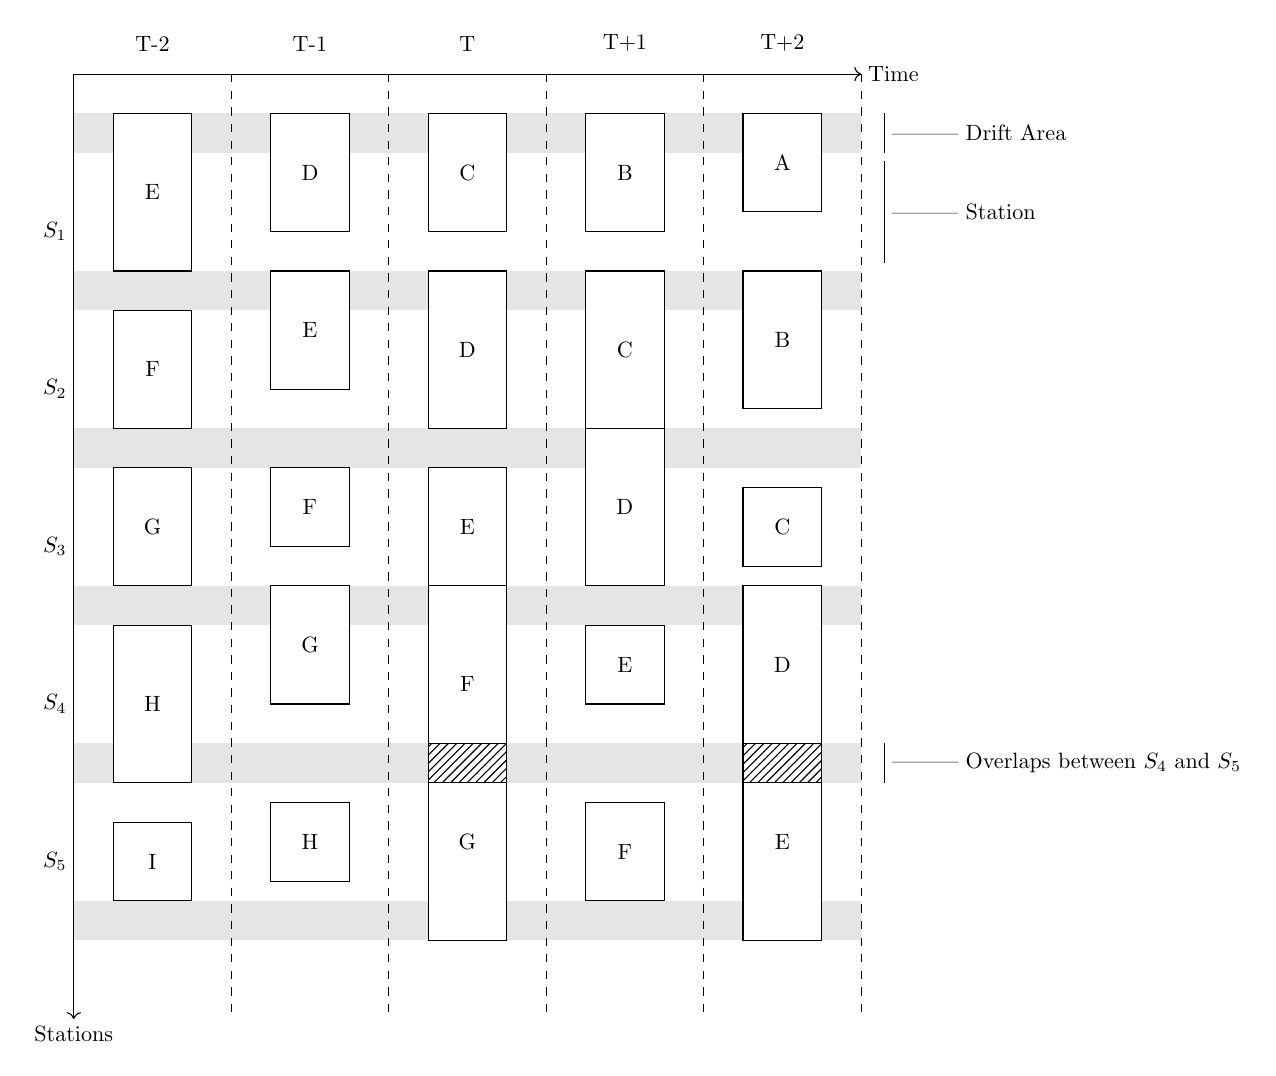
\begin{tikzpicture}[scale=1, every node/.style={scale=0.8, inner sep=3pt}]

        \foreach \y in {-1,-3,-5,-7,-9, -11} {
            \fill[gray!20] (0,\y+0.5) rectangle (10,\y);
        }

        \draw[->] (0,0) -- (10,0) node[right]{Time};
        \draw[->] (0,0) -- (0,-12) node[below]{Stations};

        \foreach \y/\name in { -2/$S_1$, -4/$S_2$, -6/$S_3$, -8/$S_4$, -10/$S_5$ } {
            \node[left] at (0,\y) { \name };
        }
        \draw[fill=white] (0.5,-9.5) rectangle (1.5,-10.5) node[midway]{I};

        \draw[fill=white] (0.5,-7) rectangle (1.5,-9) node[midway]{H};
        \draw[fill=white] (2.5,-9.25) rectangle (3.5,-10.25) node[midway]{H};

        \draw[fill=white] (0.5,-5) rectangle (1.5,-6.5) node[midway]{G};
        \draw[fill=white] (2.5,-6.5) rectangle (3.5,-8) node[midway]{G};
        \draw[fill=white] (4.5,-8.5) rectangle (5.5,-11) node[midway]{G};

        \draw[fill=white] (0.5,-3) rectangle (1.5,-4.5) node[midway]{F};
        \draw[fill=white] (2.5,-5) rectangle (3.5,-6) node[midway]{F};
        \draw[fill=white] (4.5,-6.5) rectangle (5.5,-9) node[midway]{F};
        \draw[fill=white] (6.5,-9.25) rectangle (7.5,-10.5) node[midway]{F};

        \draw[fill=white] (0.5,-0.5) rectangle (1.5,-2.5) node[midway]{E};
        \draw[fill=white] (2.5,-2.5) rectangle (3.5,-4) node[midway]{E};
        \draw[fill=white] (4.5,-5) rectangle (5.5,-6.5) node[midway]{E};
        \draw[fill=white] (6.5,-7) rectangle (7.5,-8) node[midway]{E};
        \draw[fill=white] (8.5,-8.5) rectangle (9.5,-11) node[midway]{E};

        \draw[fill=white] (2.5,-0.5) rectangle (3.5,-2) node[midway]{D};
        \draw[fill=white] (4.5,-2.5) rectangle (5.5,-4.5) node[midway]{D};
        \draw[fill=white] (6.5,-4.5) rectangle (7.5,-6.5) node[midway]{D};
        \draw[fill=white] (8.5,-6.5) rectangle (9.5,-8.5) node[midway]{D};

        \draw[fill=white] (4.5,-0.5) rectangle (5.5,-2) node[midway]{C};
        \draw[fill=white] (6.5,-2.5) rectangle (7.5,-4.5) node[midway]{C};
        \draw[fill=white] (8.5,-5.25) rectangle (9.5,-6.25) node[midway]{C};

        \draw[fill=white] (6.5,-0.5) rectangle (7.5,-2) node[midway]{B};
        \draw[fill=white] (8.5,-2.5) rectangle (9.5,-4.25) node[midway]{B};

        \draw[fill=white] (8.5,-0.5) rectangle (9.5,-1.75) node[midway]{A};

\draw[pattern=north east lines, pattern color=black] (4.5,-8.5) rectangle (5.5,-9) node[midway]{};
        
\draw[pattern=north east lines, pattern color=black] (8.5,-8.5) rectangle (9.5,-9) node[midway]{};

        \foreach \x/\label in {2/T-2, 4/T-1, 6/T, 8/T+1, 10/T+2} {
            \draw[dashed] (\x,0) -- (\x,-12);
            \node[above] at (\x-1,0.2) {\label};
        }

        \draw (10.3,-0.5) -- (10.3,-1) node[midway,right]{|---| Drift Area };
        \draw (10.3,-1.1) -- (10.3,-2.4) node[midway,right]{|---| Station };

        \draw (10.3,-8.5) -- (10.3,-9) node[midway,right]{|---| Overlaps between $S_4$ and $S_5$};


    \end{tikzpicture}
    \caption{Assembly Line Example with Uniform Station and clockcycles}
    \label{fig:assembly}
\end{figure}

    Issues in visualizing this way start to appearing when we start to consider that different stations $S_n$ and $S_m$ may take different times to complete. If we then step a clockcycle for each possible item, then we can never keep our items in sync. The main issue is that; if we compare the station $S_n$ and $S_m$, then we'll see that each station have a different time to finish, then the clockcycle system will not be perfect or even realistic as stations with differing times will each finish in different times and thus an item $X$ might make it to the station $S_{n+2}$ from $S_n$ in the same time it takes item $Y$ to make it to $S_{m+1}$ from $S_{m}$.

Thus we find the difficulty in displaying it properly in an intuitive graphical user interface. If we wish to display each station as uniform sizes, then we also have to stretch the items to make up for it visually. But doing this we have no intuitive way of knowing that $S_4$ could be 200 seconds long in real life, while $S_3$ could be 300. \textit{As luck would have it, each station in this specific case are each roughly 7 minutes long, 700cmin}, thus we will not run into any major desync problems using clockcycles on these stations.

Between each station lies a buffer zone refered to a "drift area". A drift area in this case is a transitional area between any given station $S_n$ and $S_{n+1}$. Both of the stations can borrow time from each other within this area, but only one station may utilize that area at the time. This proves useful to help fit items that take longer on some stations onto the assembly line, but these conveniences which at first glance makes this problem easier are also the source of problems that may ensue in production.

As pictured in \autoref{fig:assembly}, $D$ will take a lot of time on $S_4$ and is forced to utilize time from $S_3$ and $S_5$. 
While this works well in a vacuum, the problems start to arise when $E$ also has to utilize additional time from its neighbouring stations, causing an overlap between $D$ and $E$ at $T+2$ as they both require the use of the drift area. 

The same problem can be seen at $T$ with $F$ and $G$ as both items need to borrow time from the stations before and after. Thus we run into an overlap, as the items \textit{cannot} fit.

Do note that on $T$, $E$ does not utilize the drift area which results in it sitting flush with $F$ on the timeline, this may look good on paper but can result in overlap in practice due to the human workers at the assembly line occasionally taking a bit longer than presumed. This can be resolved by borrowing some time from $S_2$ and moving $E$ into the drift area. 

The same issue derives at $T+1$ where $C$ and $D$ just \textit{barely} get enough time, but it cannot get resolved by simply moving $D$ forward, as $D$ on $T+2$ will require all of the time it can get on $S_4$. 

\section{Jump-in and Jump-out (FIXME)}
In modern production, product sequences are typically finalized and frozen in batches before entering the assembly line. Ideally, the order remains unchanged, but last-minute adjustments may occasionally be necessary. When a product is missing critical components and cannot be built, it cannot proceed on the assembly line. In such cases, the product must be temporarily removed from the sequence and held until all parts are available, a process referred to as \emph{jump-out}.

A related challenge occurs when the missing components finally arrive. At this point, the product occupies space on the assembly station. Ideally, it should be reintegrated into the line as soon as possible, preferably before the next batch begins production. Currently, however, reintegration is delayed, and the suspended product may not re-enter the assembly line until several batches later. \cite{ref6}

From an algorithmic perspective, a \emph{jump-in} can be treated as an $O(n)$ problem: one needs only to inspect the $n$ positions in a sequence of length $n$ to determine the best insertion point in the upcoming batch. Implemented correctly, a jump-in could occur as soon as the following batch. Nevertheless, depending on operational constraints, it may not be feasible in every batch.

Jump-out, on the other hand, can be considered an $O(1)$ problem, though it presents additional practical challenges. Removing a product from the assembly line creates a gap that must be managed. This gap may require shifting a portion of the line by a clock cycle, potentially causing overloads. Alternatively, the gap could be left in place, which avoids overloading but may result in lost revenue.

\clearpage %blir fult annars
\section{Defining Drift Area}
\label{chap:drift}
The Drift Area is visualized in this thesis as a gray zone intersecting two neighbouring stations, it is also the source of our scheduling conflicts. The Drift Area allows for a lot of flexibility due to the fact that \textit{instead} of slowing down the assembly line to $1100$ Cmin and decreasing the production output by roughly $40\%$, the assembly line instead moves at a pace of $700$ Cmin per station (Standard Takt), with $200 $Cmin available as \textit{drift} on both sides.

For a station $S_n$ (where $Takt = 700$ Cmin), we can use up to $200$ Cmin from $S_{n-1}$ and up to $200$ Cmin from $S_{n+1}$. This is refered to in this thesis as \textbf{Borrowing}. Borrowing this way will give us up to a total time of $1100$ Cmin for any given task, with the caveat of $S_{n-1}$ and $S_{n+1}$ being reduced to a minimum of $500$ Cmin.

It's also important to note that while Object $n$ is borrowing from $S_{n+1}$, then work cannot begin on $n+1$ until it has finished. 


\begin{figure}[htbp]
\centering
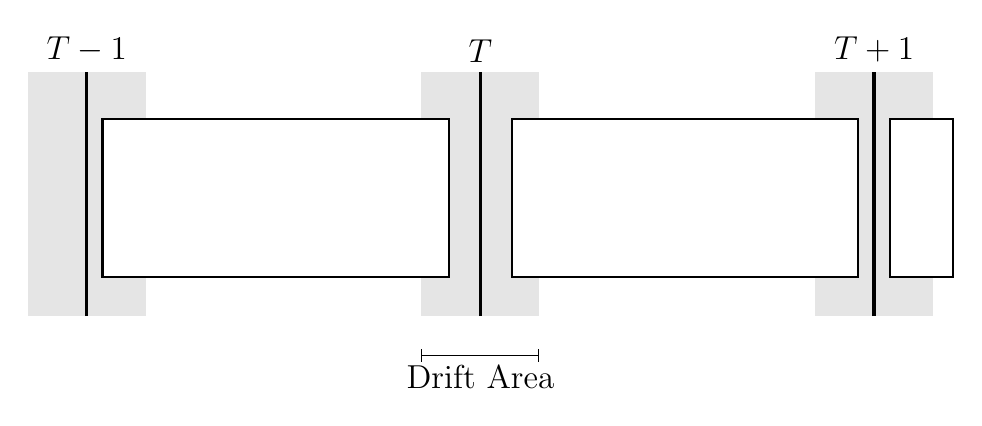
\begin{tikzpicture}[>=Latex, font=\large, scale=1, transform shape]
  \foreach \x in {0, 5, 10} {
    \fill[gray!20] (\x - 0.75, -1) rectangle (\x + 0.75, 2.1);
  }
  \draw[thick, fill=white] (0.2, -.5) rectangle (4.6, 1.5);
  \draw[thick, fill=white] (5.4, -.5) rectangle (9.8, 1.5);
  \draw[thick, fill=white] (10.2, -.5) rectangle (11.0, 1.5);
  \draw[|-|] (4.25, -1.5) -- (5.75, -1.5) node[midway, below] {Drift Area};
  
  \foreach \x/\label in {0/{$T-1$}, 5/{$T$}, 10/{$T+1$}} {
    \draw[very thick] (\x, -1) -- (\x, 2.1);
    \node[above, black] at (\x, 2.1) {\bfseries \label}; 
  }
\end{tikzpicture}
    \caption{Two objects whose $Size_{T_n} < Takt$. This is the most common case, as opposed to the more extreme cases shown in this thesis.}
\end{figure}

\begin{figure}[htbp]
\centering
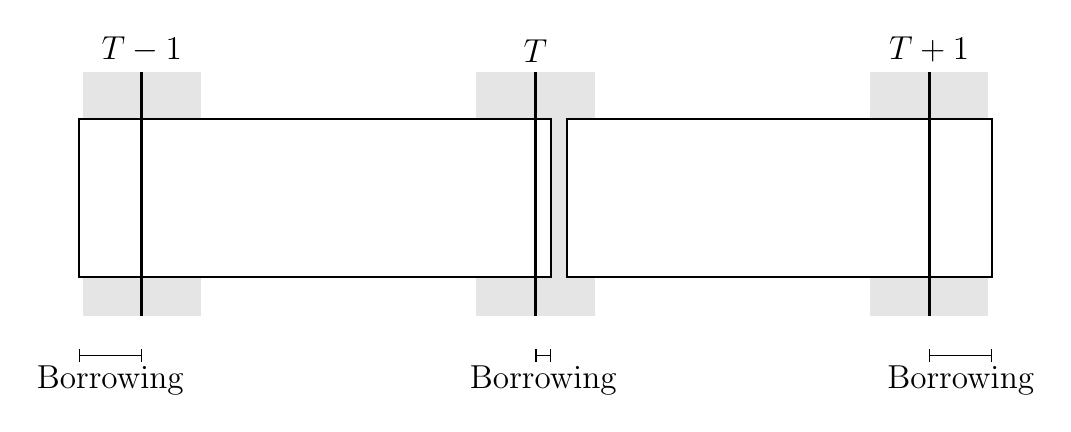
\begin{tikzpicture}[>=Latex, font=\large, scale=1, transform shape]
  \foreach \x in {0, 5, 10} {
    \fill[gray!20] (\x - 0.75, -1) rectangle (\x + 0.75, 2.1);
  }
  \draw[thick, fill=white] (-0.8, -.5) rectangle (5.2, 1.5);
  \draw[thick, fill=white] (5.4, -.5) rectangle (10.8, 1.5);
  \draw[|-|] (-.8, -1.5) -- (0, -1.5) node[midway, below] {Borrowing};
  \draw[|-|] (5, -1.5) -- (5.2, -1.5) node[midway, below] {Borrowing};
  \draw[|-|] (10, -1.5) -- (10.8, -1.5) node[midway, below] {Borrowing};
  
  \foreach \x/\label in {0/{$T-1$}, 5/{$T$}, 10/{$T+1$}} {
    \draw[very thick] (\x, -1) -- (\x, 2.1);
    \node[above, black] at (\x, 2.1) {\bfseries \label}; 
  }
\end{tikzpicture}
    \caption{Two objects whose $Size_{T_n} > Takt$. Both need to borrow time from their neighbouring stations in order to finish in time.}
\end{figure}
\section{Defining Overlaps}
\label{chap:overlap}

Overlaps stem from timing dependencies: each item’s "size" on a station $S_n$ depends on how long it takes for the item to process at the station. In other words, the "size" of the task is the duration of the task relative the duration of the station. If a task exceeds \textbf{Takt} in duration, then the use of the drift area is mandatory. 

However, if two items are processed consecutively at station $S_n$, and both of those items exceed \textbf{Takt} in $S_n$ to the point of requiring the usage of both of its neighbouring stations ($S_{n-1}$ and $S_{n+1}$), then there \textit{will} not be sufficient time for all operations to complete if both of those objects need to borrow time. These conflicting dependencies result in what's visualized as (and defined in theis thesis as) an overlap, there simply isn't enough time for assembly to finish in time.

In practice the items do not literally stack or collide. Rather, the assembly line must halt in order to allow the operation to complete before the assembly line may continue again. 

Overlap are simply put how station overloads are visualized in this thesis, as we follow the constraint that no matter what, an allocation can never exceed $Takt + 2 * Drift$ in size, and an allocation can never go past the right-most limit of the drift area on the coming station.


\begin{figure}[htbp]
\centering

\begin{minipage}{0.45\textwidth}
\centering
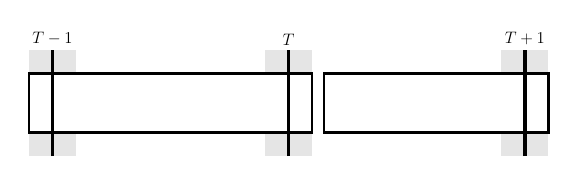
\begin{tikzpicture}[>=Latex, font=\large, scale=0.5, transform shape]

  \foreach \x in {0, 6, 2*6} {
    \fill[gray!20] (\x - 1.2/2, -0.6) rectangle (\x + 1.2/2, 1.5 + 0.6);
  }

  \draw[thick, fill=white] (-0.6, 0) rectangle (6 - 1.2/2+1.2, 1.5);
  
  \draw[thick, fill=white] (6 - 1.2/2+1.5, 0) rectangle (6*2 + 1.2/2, 1.5);

  \foreach \x/\label in {0/{$T-1$}, 6/{$T$}, 2*6/{$T+1$}} {
    \draw[very thick] (\x, -0.6) -- (\x, 1.5 + 0.6);
    \node[above, black] at (\x, 1.5 + 0.6) {\bfseries \label}; 
  }

\end{tikzpicture}
\caption{An example of two allocations, where there is enough room to borrow time for the larger one.}
\end{minipage}\hfill
\begin{minipage}{0.45\textwidth}
\centering
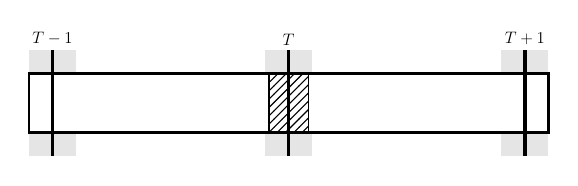
\begin{tikzpicture}[>=Latex, font=\large, scale=0.5, transform shape]

  \foreach \x in {0, 6, 2*6} {
    \fill[gray!20] (\x - 1.2/2, -0.6) rectangle (\x + 1.2/2, 1.5 + 0.6);
  }

  \draw[thick, fill=white] (-.6, 0) rectangle (6 + 0.5, 1.5);
  
  \draw[thick, fill=white] (6 - 0.5, 0) rectangle (2*6 + 1.2/2, 1.5);

  \draw[pattern=north east lines, pattern color=black] (6 - 0.5, 0) rectangle (6 + 0.5, 1.5);

  \foreach \x/\label in {0/{$T-1$}, 6/{$T$}, 2*6/{$T+1$}} {
    \draw[very thick] (\x, -0.6) -- (\x, 1.5 + 0.6);
    \node[above, black] at (\x, 1.5 + 0.6) {\bfseries \label};
  }

\end{tikzpicture}
\caption{An example of two allocations, where there is not enough room as both require borrowing, causing an overlap.}
\end{minipage}

\end{figure}

\chapter{State of the Art Analysis}
\label{ch:sota}


The Mixed-Model Assembly Line (MMAL) problem is an optimization problem, formally classified as NP-Hard. Traditionally, these optimization problems are addressed using heuristic or meta-heuristic algorithms, rather than using machine learning.

In recent years, Deep Reinforcement Learning (DRL) has become a dominant approach for solving dynamic scheduling problems. Unlike supervised methods, DRL agents learn through trial-and-error interaction with a simulation environment, aiming to maximize a cumulative reward signal.

For example, Chen et al. proposed an Adaptive Deep Q-Network, which builds on the Q-Learning Agorithm in order to address scheduling in Cloud Manufacturing environments characterized by random task arrivals. Their approach utilizes a resizable network structure to adapt to changing machine availability and employs a complex reward mechanism to balance multiple objectives, such as minimizing work time, and optimizing machine load. \cite{ref10} 

However, reinfocement learning requires trying and failing repeatedly in order to learn, and applying such trial and error Reinforcement Learning methods to a Mixed-Model Assembly Line (MMAL), especially in a production environment, will pose significant risks. In a cloud environment, a scheduling error typically results in a slowdown in the form of increased latency or reduced throughput. In contrast, a scheduling error in a physical MMAL situation often results in scheduling overlaps that force the entire assembly line to halt in order for each station to be able to finish in time. Given these higher stakes, the exploratory nature of reinforcement learning agents may be prohibitively costly compared to imitating provene human strategies, hence the use of Deep Unsupervised Learning was chosen instead.

While DRL is effective for dynamic environments where rules change frequently, it presents significant implementation challenges. It requires the construction of a high-fidelity simulation environment and the careful engineering of state and action spaces. Furthermore, the "black box" nature of the reward signal makes it difficult to capture the nuanced, unwritten knowledge of the human servicemen, which is the primary objective of this thesis.

Current manual approaches rely heavily on the "tacit knowledge" of management staff, knowledge accumulated through experience that is difficult to articulate as explicit rules, especially if rules have accumulated over time. This thesis proposes capturing this knowledge using Supervised Learning, formally known in this context as Imitation Learning. 


\section{Recurrent Architectures}
\label{sec:recurrent_arch}

To emulate the sequential decision-making process of human schedulers, we first investigate architectures adapted from Natural Language Processing (NLP) that process data sequentially.

\subsection{Long Short-Term Memory (LSTM)}
\label{subsec:lstm}

In previous works addressing similar scheduling problems, researchers have applied Recurrent Neural Networks (RNNs), often utilizing Long Short-Term Memory (LSTM) units within a sequence-to-sequence (Seq2Seq) framework \cite{ref2}.

A defining characteristic of LSTMs is their ability to selectively forget irrelevant or outdated information via the "forget gate". This mechanism allows the model to focus on relevant patterns over time, mitigating the vanishing gradient problem inherent in standard RNNs and improving the modeling of long-term dependencies \cite{ref4, ref9}.

\subsection{Sequence-to-Sequence (Seq2Seq) Models}

Seq2Seq models, typically built upon encoder-decoder RNN architectures, are designed to map an input sequence to an output sequence of a different length or order \cite{ref2}.  While traditionally applied to machine translation (e.g., transforming English to Swedish), this architecture is adaptable to the assembly line problem. In this context, the input is a sequence of vectorized product orders, and the output is the permuted production sequence \cite{ref3}.

However, applying standard Seq2Seq models to permutation problems presents a specific challenge: \textbf{vocabulary definition}. Standard NLP models select outputs from a fixed, pre-defined vocabulary, similar to a dictionary. In a manufacturing context, where every day's product list is unique, a fixed vocabulary is insufficient. The model must instead learn to select from the dynamic input available that day, a task that is non-trivial for standard Seq2Seq architectures unless they strictly rely on abstract sequence indices \cite{ref2, ref3}.

One way to remedy this limitation is to modify the decoder to point directly to the input elements, an approach that leads to the development of Pointer Networks (discussed in Section \ref{subsec:pointer_nets}).

\subsection{Limitations of Recurrent Architectures}

Despite their historical success, RNN and LSTM-based models suffer from a significant bottleneck: \textbf{sequential processing}. This is because these models must process the input sequence step-by-step, so that item $t$ depends on item $t-1$, they cannot parallelize computation either. This results in slower training times and, more importantly, a limited ability to capture a lot of global context across the entire schedule simultaneously \cite{ref4}.

This limitation motivates the shift toward \textbf{Attention-based approaches}, which process the entire sequence in parallel, and has a larger global context scope.

\section{Attention-Based Architectures}
\label{sec:attention_arch}

\subsection{The Transformer Model}
\label{subsec:transformer}

To address the sequential bottlenecks of RNNs, Transformer-based architectures discard recurrence entirely, relying instead on a self-attention mechanism \cite{ref5}.

The defining characteristic of the Transformer is the use of scaled dot-product attention. This allows the model to weigh the importance of each element in a given sequence relative to all other elements in that same sequence, regardless of distance. \cite{ref14} This parallelized computation not only accelerates training but enables the model to capture global dependencies more effectively than RNN-based methods. Since Transformers are order-agnostic, positional encodings are added to the input vectors to retain sequence order information \cite{ref5}.

For combinatorial scheduling problems, this translates into the ability to model complex interactions across the entire planning horizon. \cite{ref13} The placement of one item can be directly conditioned on all others in the same day's sequence, providing the context awareness necessary for effective assembly line scheduling \cite{ref8}.

\subsection{Pointer Networks}
\label{subsec:pointer_nets}

While Transformers excel at context, they still typically rely on generating tokens from a fixed vocabulary. The \textbf{Pointer Network} is the only architecture in this analysis specifically designed for combinatorial optimization and permutation problems \cite{ref7}.

Implemented using an encoder-decoder structure of the sequence-to-sequence model, the Pointer Network utilizes a specialized attention mechanism to generate context vectors that "point" to specific elements in the input sequence rather than predicting a value from a dictionary. 

This model is explicitly designed with combinatorial problems in mind, such as the traveling salesman problem, convex hull, and other combinatorial optimization problems. \cite{ref7} It can thus be used to well-suited for the mixed-model assembly line problem (MMAL), as the object attributes (such as station order, or time to complete) are immutable, and the only thing that matters for our case is the permutation/rearrangement.


\chapter{Methodology}

\section {Data generation}
\subsection{Constants}
For data generation the following constants are used:
\begin{table}[htbp]
    \centering
    \caption{Table of Constants used in Data Generation}
    \label{tab:generation_constants}
    \begin{tabular}{l c l} % Left-aligned, Centered, Left-aligned
        \toprule
        \textbf{Constant} & \textbf{Default Value} & \textbf{Description} \\ 
        \midrule
        Objects    & 100     & Total number of objects in the testing sequence \\
        Stations   & 35      & Number of stations \\
        Takt       & 700     & The cycle time ($Cmin$) \\
        Drift      & 200     & The size of the drift area ($Cmin$) \\
        Gap        & 10       & Minimum buffer distance between objects \\
        Multiplier & 500     & Constant value to multiply \textit{Objects} with \\
        \bottomrule
    \end{tabular}
\end{table}
\subsection{Data Preprocessing and Abstraction}
For the purpose of training optimization, the raw information is abstracted into a concise JSON schema. Each entry in the dataset is reduced to the following three attributes:

\begin{itemize}
    \item \textbf{Object ID} (\texttt{object}): An integer representing the unique identifier of the item.
    \item \textbf{Station Data} (\texttt{data}): A mapping of station keys ($s_1, \dots, s_{35}$) to their respective time requirement values.
    \item \textbf{Station Offsets} (\texttt{offsets}): A mapping of station keys to their relative offset values.
\end{itemize}

By utilizing these values, we can train a model to prioritize time-based decision-making over rigid rule-based systems. It is important to note that while the model operates without explicit constraints, the use of a sufficiently large dataset derived from expert tacit knowledge ensures that it implicitly adheres to fundamental ground rules, albeit with greater flexibility.

\subsection{Offset Calculation and Centering}
The positioning of an object within a station is determined by its \textit{offset} relative to the \textbf{Takt} start ($0$ locally). The script employs a dynamic centering logic that positions tasks within the remaining available capacity of the standard Takt window. This approach balances the empty space (or buffer) on either side of the allocation, adapting to the finish time of the preceding task.

To determine the position, the script first calculates the local start time, $t_{start}$, which corresponds to the completion of the previous allocation relative to the current Takt. The remaining buffer, $B$, is calculated as the difference between the standard Takt duration $T$ and the occupied time, clamped to zero to ensure non-negative spacing:

\begin{equation}
    B = \max(0, T - t_{start} - S)
\end{equation}

Where $S$ is the size (duration) of the new task. The tentative offset, $O_{calc}$, is then derived by placing the task at the start position plus half of the calculated buffer:

\begin{equation}
    O_{calc} = t_{start} + \frac{B}{2}
\end{equation}

This formula ensures that if the previous task finishes early, the new task is centered in the wide gap; if the previous task finishes late, the buffer shrinks, effectively pulling the new task closer to the previous one.

Finally, to ensure the object adheres to physical station boundaries and drift limitations ($D$), the calculated offset is clamped. The maximum permissible offset is defined such that the task end does not exceed the drift limit ($T+D$):

\begin{equation}
    O_{calc} = \max(-D, \min(O_{calc}, T + D - S))
    \label{eq:offset_constraint}
\end{equation}

\begin{figure}[htbp]
\centering

\begin{minipage}{0.48\textwidth}
\centering
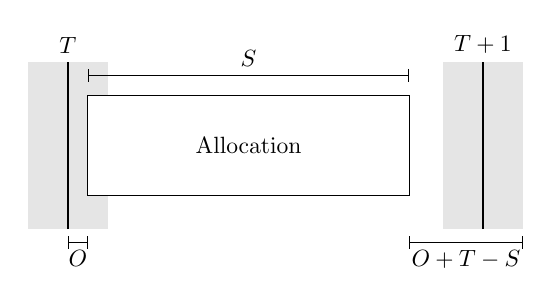
\begin{tikzpicture}[>=Latex, scale=0.85, transform shape]

  \fill[gray!20] (-1.2, -0.5) rectangle (0, 2);

  \fill[gray!20] (5, -0.5) rectangle (6.2, 2);

  \draw[draw, fill=white] (-0.3,0) rectangle (4.5, 1.5) node[pos=.5] {Allocation};

  \draw[thick] (-0.6, -0.5) -- (-0.6, 2);
  \draw[thick] (5.6, -0.5) -- (5.6, 2);

  \node[above] at (-0.6, 2) {$T$};
  \node[above] at (5.6, 2) {$T+1$};

  \draw[|-|] (-0.3, 1.8) -- (4.5, 1.8) node[midway, above] {$S$};

  \draw[|-|] (-0.6, -0.7) -- (-0.3, -0.7) node[midway, below] {$O$};

  \draw[|-|] (4.5, -0.7) -- (6.2, -0.7) node[midway, below] {$O + T - S$};

\end{tikzpicture}
    \caption{Allocation positioning before the centering process (FIXME)}
\end{minipage}\hfill
\begin{minipage}{0.48\textwidth}
\centering
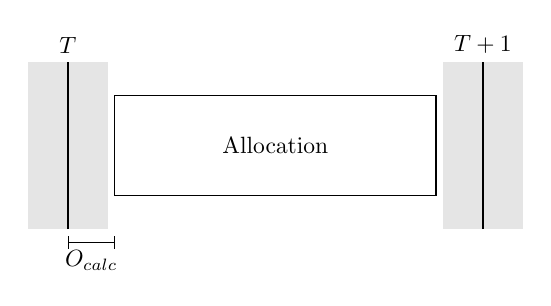
\begin{tikzpicture}[>=Latex, scale=0.85, transform shape]

  \fill[gray!20] (-1.2, -0.5) rectangle (0, 2);

  \fill[gray!20] (5, -0.5) rectangle (6.2, 2);

  \draw[draw, fill=white] (0.1,0) rectangle (4.9, 1.5) node[pos=.5] {Allocation};

  \draw[thick] (-0.6, -0.5) -- (-0.6, 2);
  \draw[thick] (5.6, -0.5) -- (5.6, 2);

  \node[above] at (-0.6, 2) {$T$};
  \node[above] at (5.6, 2) {$T+1$};

  \draw[|-|] (-0.6, -0.7) -- (0.1, -0.7) node[midway, below] {$O_{calc}$};

\end{tikzpicture}
\caption{Allocation after centering.}
\end{minipage}

\end{figure}

\subsection{Constructive Data Generation as a Solved Puzzle}

To train the machine learning model, a synthetic dataset is required that represents valid, collision-free production schedules. Rather than randomly placing tasks and checking for validity, the system employs a constructive generation algorithm. This approach acts as a forward simulation, placing allocations sequentially to inherently create a "solved puzzle" which serves as the ground truth for training.

\subsubsection*{Dependency-Based Positioning}
The placement of any given allocation $A_{i,j}$ (Object $i$ at Station $j$) is not independent. It is strictly constrained by two spatial-temporal boundaries derived from the existing grid state:
\begin{enumerate}
    \item \textbf{Station Availability:} The station $j$ must be free. Therefore, $A_{i,j}$ cannot start until the previous object $i-1$ has departed station $j$.
    \item \textbf{Object Availability:} The object $i$ must be ready. Therefore, $A_{i,j}$ cannot start until object $i$ has finished processing at the previous station $j-1$.
\end{enumerate}

Mathematically, the earliest valid start time ($t_{start}$) for the new allocation is defined as the maximum of these two completion timestamps, plus a configured safety gap:

\begin{equation}
    t_{start} = \max(End_{i-1, j}, \quad End_{i, j-1}) + Gap
\end{equation}

This logic ensures that the generated schedule is causally valid—no object effectively "teleports" between stations, and no two objects overlap on a single station.

\subsubsection*{Context-Aware Scaling}
The dimensions of the tasks are also generated dependently. While a desired duration is chosen stochastically, the actual assigned size ($S$) is clamped by the remaining available time in the Takt window. The generator calculates the available space between the calculated $t_{start}$ and the maximum drift boundary. If the random size exceeds this space, it is truncated to fit.

This process results in a dataset where every input (the sequence of objects) has a perfectly matching output (the offsets and sizes) that is guaranteed to be solvable, providing a robust target for supervised learning.

(FIXME)

\begin{figure}[H] 
\centering
\begin{minipage}{0.48\textwidth}
    \centering
    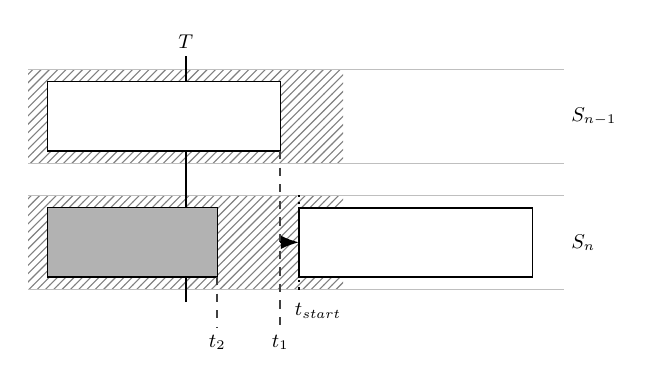
\begin{tikzpicture}[>=Latex, font=\small, scale=0.8, transform shape]

        \fill[pattern=north east lines, pattern color=gray] (-2.5, 2.0) rectangle (2.5, 3.5);
        \fill[pattern=north east lines, pattern color=gray] (-2.5, 0) rectangle (2.5, 1.5);
        \draw[gray!50] (-2.5, 2.0) -- (6, 2.0);
        \draw[gray!50] (-2.5, 3.5) -- (6, 3.5);
          
        \draw[gray!50] (-2.5, 0) -- (6, 0);
        \draw[gray!50] (-2.5, 1.5) -- (6, 1.5);

        % Added Station Labels
        \node[right] at (6, 2.75) {$S_{n-1}$};
        \node[right] at (6, 0.75) {$S_{n}$};

        \draw[thick] (0, -0.2) -- (0, 3.7);
        \node[above] at (0, 3.7) {$T$};
        \draw[fill=white, draw=black] (-2.2, 2.2) rectangle (1.5, 3.3);

        \draw[thick, dashed, darkgray] (1.5, 2.2) -- (1.5, -0.6);
        \node[below] at (1.5, -0.6) {$t_{1}$};

        \draw[fill=gray!60, draw=black] (-2.2, 0.2) rectangle (0.5, 1.3);

        \draw[thick, dashed, darkgray] (0.5, 0.2) -- (0.5, -0.6);
        \node[below] at (0.5, -0.6) {$t_{2}$};
         
        \draw[fill=white, draw=black, thick] (1.8, 0.2) rectangle (5.5, 1.3);
        \fill[white] (5.2, 0.22) rectangle (5.5, 1.28);
         
        \node[font=\bfseries] at (3.65, 0.75) {};

        \draw[->, thick, black] (1.5, 0.75) -- (1.8, 0.75);
        \draw[dotted, thick] (1.8, 0) -- (1.8, 1.5);
        \node[below] at (2.1, -0.1) {$t_{start}$};

    \end{tikzpicture}
    \caption{Case 1: The white object in $S_{n-1}$ is borrowing time from itself at $S_n$, and thus cannot begin assembly at $S_n$ until it has finished the task at $S_{n-1}$.}
\end{minipage}\hfill
\begin{minipage}{0.48\textwidth}
    \centering
    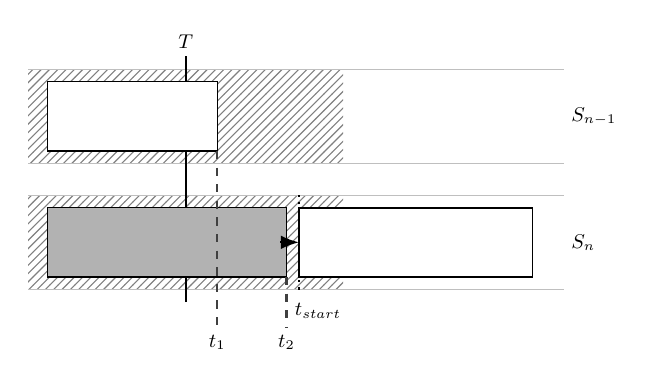
\begin{tikzpicture}[>=Latex, font=\small, scale=0.8, transform shape]

        \fill[pattern=north east lines, pattern color=gray] (-2.5, 2.0) rectangle (2.5, 3.5);
        \fill[pattern=north east lines, pattern color=gray] (-2.5, 0) rectangle (2.5, 1.5);
        \draw[gray!50] (-2.5, 2.0) -- (6, 2.0);
        \draw[gray!50] (-2.5, 3.5) -- (6, 3.5);
          
        \draw[gray!50] (-2.5, 0) -- (6, 0);
        \draw[gray!50] (-2.5, 1.5) -- (6, 1.5);

        % Added Station Labels
        \node[right] at (6, 2.75) {$S_{n-1}$};
        \node[right] at (6, 0.75) {$S_{n}$};

        \draw[thick] (0, -0.2) -- (0, 3.7);
        \node[above] at (0, 3.7) {$T$};
        \draw[fill=white, draw=black] (-2.2, 2.2) rectangle (0.5, 3.3);


        \draw[fill=gray!60, draw=black] (-2.2, 0.2) rectangle (1.6, 1.3);
          
        \draw[fill=white, draw=black, thick] (1.8, 0.2) rectangle (5.5, 1.3);
        \fill[white] (5.2, 0.22) rectangle (5.5, 1.28);
          
        \node[font=\bfseries] at (3.65, 0.75) {};

        \draw[thick, dashed, darkgray] (.5, 2.2) -- (.5, -0.6);
        \node[below] at (.5, -0.6) {$t_{1}$};

        \draw[thick, dashed, darkgray] (1.6, 0.2) -- (1.6, -0.6);
        \node[below] at (1.6, -0.6) {$t_{2}$};

        \draw[->, thick, black] (1.5, 0.75) -- (1.8, 0.75);
        \draw[dotted, thick] (1.8, 0) -- (1.8, 1.5);
        \node[below] at (2.1, -0.1) {$t_{start}$};

    \end{tikzpicture}
    \caption{Case 2: The gray object is borrowing time from the white object in $S_n$. Even though it finished in $S_{n-1}$, the white object cannot begin assembly right away in $S_n$ as it's dependent on the gray object finishing at $S_n$.}
\end{minipage}
\end{figure}
\section{JSON to Vector Methodology}
Machine learning models operate on numerical vector data, often represented as \textit{tensors}, rather than on raw JSON structures. Given a list of JSON objects on an assembly line, each JSON can be encoded into a fixed-length vector $x_t$ by extracting and normalizing its features. This process transforms the entire list into a sequence of vectors ${[x_1, x_2, \dots, x_N]}$. Using sequences from historical data, a model can then be trained to learn a mapping from an input order of JSONs to a desired output order.

\section{Transforming a language-based model into a sequence based model}

Two of the models examined in this thesis were originally designed for natural language processing tasks, such as translation between different languages. Both these models rely on a predefined vocabulary, which can prove problematic when not handling regularly occuring words, but rather unique objects of differing properties. This raises the question of whether a list of products can be treated analogously to a collection of words where each product variation forms a distinct element within the vocabulary. Doing so could allow the model to more accurately replicate historical data, along with its flaws.

However, certain constraints must be imposed as language models often overproduce common tokens such as “the,” since these words are statistically more likely to appear in most positions in any given English sentence. To avoid this bias, the model must instead operate on genuine rearrangements or permutations relevant to our specific application. This can be done using Embedding. (See \ref{chap:workarounds})

\subsection{Workarounds}
\label{chap:workarounds}

To adapt the architecture of Natural Language Processing for product sequencing without suffering from the previously mentioned limitations, two specific architectural modifications were implemented:

\subsubsection{Continuous-Discrete Embedding}
Standard NLP models map a finite set of words to static vectors. Since product variations are continuous rather than discrete, a traditional vocabulary approach would require an infinite vocabulary size to capture every possible variation.

To resolve this, the implementation utilizes a custom \textit{ObjectEmbedding} layer. The discrete station identifier is mapped via a standard lookup table, while the size value is projected through a linear layer. These two feature sets are concatenated to form the input vector:
\begin{equation}
E_{input} = \text{Concat}(\text{Embedding}(ID), \text{Linear}(Size)) %TODO: dubbelkolla
\end{equation}
This allows the attention mechanism to process the semantic identity of the station, enabling the model to generalize to unseen product sizes without expanding the vocabulary.

\subsubsection{Decoupling Prediction from Sequencing}
\label{subp:decoupling}
To strictly prevent the common issue of repeting tokens in generative language models, and instead repurpose it for permutation, the sequence generation decoupled from the neural network entirely.

The language models are configured as standalone Encoders, serving purely as a regressor to predict the offsets of each station. It does not output a probability distribution over the next token. Instead, the final reordering is performed by a combinatorial optimizer (Simulated Annealing) which utilizes the predictions to minimize a conflict cost matrix:
\begin{equation}
\text{Cost}_{ij} = \sum (\max(0, | \text{Drift}_i | + | \text{Drift}_j | - \text{Limit}))^2 %TODO: dubbelkolla
\end{equation}

By using the language models solely for feature extraction, and delegating the sorting logic to mathematics, the system ensures that the output is always a valid permutation of the input, which will guarantuee that no items become duplicated or omitted.

\chapter{System Architecture}

\section{Machine Learning Models}

\begin{table}[htbp]
    \centering
    \caption{Table of Constants used for Machine Learning (Excluding paths)}
    \label{tab:generation_constants}
    \begin{tabular}{l c} % Left-aligned, Centered, Left-aligned
        \toprule
        \textbf{Constant} & \textbf{Default Value} \\ 
        \midrule
        batch\_size &  $16$ \\
        num\_epochs & $10$ \\
        lr & $1e^{-4}$ \\
        d\_model & $128$ \\
        dropout & $0.1$ \\
        \bottomrule
    \end{tabular}
\end{table}

\subsection{The Transformer Model (FIXME)}
\label{sec:trans}

The architecture utilized in this thesis is derived from the canonical Transformer model proposed by Vaswani et al. \cite{ref5}, but includes significant modifications tailored to the Mixed-Model Assembly Line (MMAL) problem. Unlike standard NLP implementations that process tokenized text, this model treats the assembly line as a sequence of station-workload pairs. 

To handle this multi-modal input, the model is fitted with a custom \textit{Object Embedding} layer. As defined in the system implementation, this layer fuses categorical data with continuous variables: the station index is mapped to a learnable embedding vector of size $d_{model}/2$, while the continuous workload size is projected via a linear layer to match this dimension. These two representations are concatenated and summed with sinusoidal positional encodings, allowing the model to interpret both the magnitude of the work and its sequential position in the line.

\subsubsection{Encoder-Only Regression}
\label{subp:decoupling}
During preliminary feasibility testing, empirical results indicated that a standard Sequence-to-Sequence (Encoder-Decoder) framework was ill-suited for the regression nature of cost estimation. Consequently, the architecture was simplified to an Encoder-only configuration, conceptually similar to BERT. \cite{ref12}

In the inference pipeline, the decoder is bypassed entirely. The input sequence is processed solely by the Encoder stack to generate contextual representations, which are then passed directly to a linear projection layer. This layer outputs a scalar value for each station, representing the predicted drift offset, rather than generating a probability distribution over a vocabulary.

\subsubsection{Simulated Annealing and Cost Logic} 
While the Transformer predicts the local drift impact of individual items, the global sequence scheduling is optimized using Simulated Annealing. This method explores the solution space of item permutations to minimize line stoppage risks.

The optimization relies on a specialized cost matrix derived from the Transformer's predictions. The cost between two products, $A$ and $B$, is calculated using a "slack centering" heuristic. The system simulates the placement of product $B$ relative to product $A$ such that $B$ is centered within the available slack time, calculated as:
$$
\text{Offset}_B \approx \frac{\text{Offset}_A + \text{Size}_A - \text{Size}_B}{2}
$$
A penalty is incurred only if this simulated position violates the drift boundaries (defined as $[-Drift, Takt + Drift]$). To aggressively discourage valid-but-risky sequences, these violations are penalized quadratically ($violation^2$). By allowing for probabilistic acceptance of sub-optimal transitions, Simulated Annealing avoids the local optima that typically constrain greedy algorithms, resulting in a robust assembly line schedule.



\subsection{The Sequence-to-Sequence Model (FIXME)}
\label{sec:seq}

To establish a baseline for performance, we implemented a standard Sequence-to-Sequence (Seq2Seq) architecture tailored for regression. Unlike the Transformer approach which focuses on global context via self-attention, this model relies on Recurrent Neural Networks (RNNs) to process the station workload sequentially. The model operates as a "cost estimator," predicting the cumulative offset for a given sequence of stations, which is subsequently optimized using Simulated Annealing, as employed by the Transformer.

\subsubsection{Feature Representation}
Before entering the recurrent layers, the raw station data is processed to combine categorical identities with continuous workload values. As defined in the wrapper implementation:
\begin{itemize}
    \item \textbf{Station Embedding:} The discrete station indices are passed through a learned embedding layer to capture latent station characteristics.
    \item \textbf{Size Projection:} The continuous size values (workload) are projected through a linear layer to match the embedding dimension.
    \item \textbf{Fusion:} These two feature sets are concatenated and passed through a projection layer to form the final input vector $x_t$ of dimension $d_{model}$.
\end{itemize}

\subsubsection{Encoder-Decoder Architecture}
The core architecture consists of two Long Short-Term Memory (LSTM) networks:
\begin{itemize}
    \item \textbf{Encoder:} The encoder processes the input sequence $X = \{x_1, \dots, x_T\}$ and produces a sequence of hidden states $H = \{h_1, \dots, h_T\}$. It captures the temporal dependencies of the assembly line workload.
    \item \textbf{Decoder:} The decoder operates autoregressively. At each time step $t$, it predicts the drift value based on its previous hidden state, the previous output, and a context vector $c_t$ derived from the encoder's output.
\end{itemize}

\subsubsection{Attention Mechanism}
To mitigate the information bottleneck inherent in fixed-length vector encoding, the model utilizes an additive attention mechanism (Bahdanau Attention). For a decoder hidden state $s_{t-1}$ and encoder hidden states $h_j$, the attention energy $e_{tj}$ is calculated as:
\begin{equation}
    e_{tj} = v^T \tanh(W [s_{t-1}; h_j])
\end{equation}
where $W$ and $v$ are learnable parameters. These scores are normalized via softmax to produce attention weights $\alpha_{tj}$, which are used to compute the context vector $c_t$:
\begin{equation}
    c_t = \sum_{j=1}^{T} \alpha_{tj} h_j
\end{equation}
This context vector allows the decoder to "focus" on specific stations in the input sequence that are most relevant for predicting the current drift value.

\subsubsection{Simulated Annealing}
Like the Transformer, the Seq2Seq model is strictly used to estimate the number of conflicts. The actual optimization is handled by Simulated Annealing. The algorithm repeatedly swaps items in the sequence and uses the model to predict overlaps. It then accepts or rejects these changes based on a cooling schedule to avoid getting stuck in local minima.




\subsection{The Pointer Network Model}
The proposed solution implements a Pointer Network architecture similar to the one proposed in (O. Vinyals et al, 2015). The model essentially follows a standard Encoder-Decoder structure enhanced with a content-based attention mechanism, designed to handle variable-length input sequences and output a permutation of the input indices. 

\subsubsection{Encoder Mechanism}
The encoder processes the input sequence to generate a representation of the initial problem state.
\begin{enumerate}
    \item \textbf{Input Projection:} Raw input features are first passed through a projection block consisting of a linear layer, a $tanh$ function, and Layer Normalization. This maps the input dimension to a higher-dimensional latent space ($d_{model}$).

    \item \textbf{Bidirectional LSTM:} The projected features are fed into a Bi-directional LSTM. This allows the model to capture context from both past and future states in any given sequence. The final hidden states of the forward and backward passes are combined to form the initial context for the decoder.
\end{enumerate}

\subsubsection{Decoder and Attention Mechanism}
The decoder generates the output sequence one item at a time. Unlike standard NLP models that generate new tokens from a fixed vocabulary, this decoder selects indices from the input sequence.
\begin{itemize}
    \item \textbf{State Initialization:} The decoder's initial hidden and cell states are initialized by projecting the final concatenated states of the encoder through learnable linear "bridge" layers.
    \item \textbf{Glimpse Mechanism:} To improve the the attention mechanism, the model employs a "glimpse" step. At every time step, the decoder's current state queries the encoder outputs to calculate a context vector. This vector summarizes the most relevant parts of the input sequence for the current step.
    \item \textbf{Pointer Selection:} The final selection is performed by a second attention layer. This layer combines the decoder's current state with the context vector from the glimpse step to compute a probability distribution over the input elements. The element with the highest probability is selected as the next index in the sequence.
\end{itemize}

\subsubsection{Masking and Inference}
To ensure the validity of the resulting permutation, a masking mechanism is applied during inference. Once an input index is selected, it is masked out by setting its log-probability to $-\infty$, this will prevent the model from selecting the same element twice. The selected element's embedding is then used as the input for the next decoder time step.

\subsubsection{The Dataset}
To enable the Pointer Network to process the production schedules, the raw JSON data is transformed into structured numerical tensors through a custom preprocessing pipeline. This pipeline is responsible for extracting the relevant features from each object, normalizing the station processing times, and organizing the sequences into batches for efficient model training. (FIXME)
\begin{itemize}
    \item \textbf{Tensor Representation} \\
    Each input sequence is converted into a numerical tensor of shape $(L, N)$, where $L$ denotes the sequence length (number of objects) and $N$ corresponds to the normalized processing times for each station ($S_1$, \dots, $S_N$). For batch processing on the GPU, these tensors are padded to a uniform length $L_{max}$ and stacked, resulting in a final input structure of dimensions $(B, L_{max}, N)$, where $B$ represents the batch size.

    \item \textbf{Propagation and Usage} \\
    Upon entering the Pointer Network, this raw feature tensor is first processed by the \textit{Projector} module. A linear layer expands the input dimension $S$ into a higher-dimensional latent representation ($d_{model}$). This projected embedding is subsequently passed through a \texttt{Tanh} activation and \texttt{LayerNorm} before being consumed by the Bidirectional LSTM encoder, which generates the context-aware hidden states required for the attention mechanism.
\end{itemize}

\section{The Training Loop}
(FIXME), (see \ref{chap:workarounds})
\subsection{The Pointer Network}
    TODO
\subsection{The Transformer Model}
    TODO
\subsection{The Sequence-To-Sequence Model} 
    TODO

\section{The Application Programming Interface (API)}
The system exposes its core functionalities through a RESTful API, facilitating programmatic interaction with the implemented neural architectures. This interface serves as the primary gateway for data ingestion and inference execution.

\subsection{Endpoints}

\subsubsection{/run/\{model\_type\}}

This POST endpoint provides a unified interface for sequence processing across different model architectures (\textbf{Transformer}, \textbf{Pointer Network}, or \textbf{Seq2Seq}). Once selected it returns a processed sequence made from the input data, including refitting. 

\subsubsection{/run/\{model\_type\}/$int:n$/}

This POST endpoint is the same as the one above it, but it accepts an integer $n$, which runs the model $n$ times and returns $n$ suggested sequences. (FIXME)


\subsubsection{/check/}

This POST endpoint will count the number of \textbf{overlaps} on a given sequence, based on configuration data. 


\chapter{Experiments and results}
\section{Task Performance}
Performance is measured by how well the model can take an input with overlapping data and rearrange the tasks to minimize overlaps. The reduction metric is defined at \ref{sec:eval}.

Although the operational constraints of the target problem typically limit sequences to batches of roughly 100 objects, the following results also evaluate the model's scalability beyond this range.

\subsection{Pointer Network Performance}

\begin{table}[H]
    \centering
    \small 

    \begin{minipage}[t]{0.48\textwidth}
        \centering
        \caption{Test-size of $10$}
        \label{tab:res_10}
        \begin{tabular}{l c c}
            \toprule
            \textbf{Run} & \textbf{Ratio ($R$)} & \textbf{Red.} \\
            \midrule
            Run \#1 & $1/25$ & $96\%$ \\
            Run \#2 & $0/34$ & $100\%$ \\
            Run \#3 & $2/20$ & $90\%$ \\
            \midrule
            \textbf{Avg} & & $95.3\%$ \\
            \bottomrule
        \end{tabular}
    \end{minipage}
    \hfill
    \begin{minipage}[t]{0.48\textwidth}
        \centering
        \caption{Test-size of $100$}
        \label{tab:res_100}
        \begin{tabular}{l c c}
            \toprule
            \textbf{Run} & \textbf{Ratio ($R$)} & \textbf{Red.} \\
            \midrule
            Run \#1 & $83/367$ & $77.4\%$ \\
            Run \#2 & $75/346$ & $78.3\%$ \\
            Run \#3 & $64/340$ & $81.2\%$ \\
            \midrule
            \textbf{Avg} & & $79.0\%$ \\
            \bottomrule
        \end{tabular}
    \end{minipage}

    \vspace{0.8cm} 

    \begin{minipage}[t]{0.48\textwidth}
        \centering
        \caption{Test-size of $1000$}
        \label{tab:res_100b}
        \begin{tabular}{l c c}
            \toprule
            \textbf{Run} & \textbf{Ratio ($R$)} & \textbf{Red.} \\
            \midrule
            Run \#1 & $1121/5530$ & $79.73\%$ \\
            Run \#2 & $1128/5392$ & $79.08\%$ \\
            Run \#3 & $1233/5513$ & $77.63\%$ \\
            \midrule
            \textbf{Avg} & & $79.0\%$ \\
            \bottomrule
        \end{tabular}
    \end{minipage}
    \hfill
    \begin{minipage}[t]{0.48\textwidth}
        \centering
        \caption{Test-size of $10000$}
        \label{tab:res_100c}
        \begin{tabular}{l c c}
            \toprule
            \textbf{Run} & \textbf{Ratio ($R$)} & \textbf{Red.} \\
            \midrule
            Run \#1 & $11519/54162$ & $78.73\%$ \\
            Run \#2 & $11544/54419$ & $78.79\%$ \\
            Run \#3 & $11605/55066$ & $78.93\%$ \\
            \midrule
            \textbf{Avg} & & $78.82\%$ \\
            \bottomrule
        \end{tabular}
    \end{minipage}
\end{table}


\subsection{Transformer Performance}

\begin{table}[H]
    \centering
    \small 

    \begin{minipage}[t]{0.48\textwidth}
        \centering
        \caption{Test-size of $10$}
        \label{tab:res_10}
        \begin{tabular}{l c c}
            \toprule
            \textbf{Run} & \textbf{Ratio ($R$)} & \textbf{Red.} \\
            \midrule
            Run \#1 & $53/63$ & $15.87\%$ \\
            Run \#2 & $52/57$ & $8.77\%$ \\
            Run \#3 & $49/49$ & $0\%$ \\
            \midrule
            \textbf{Avg} & & $8.21\%$ \\
            \bottomrule
        \end{tabular}
    \end{minipage}
    \hfill
    \begin{minipage}[t]{0.48\textwidth}
        \centering
        \caption{Test-size of $100$}
        \label{tab:res_100}
        \begin{tabular}{l c c}
            \toprule
            \textbf{Run} & \textbf{Ratio ($R$)} & \textbf{Red.} \\
            \midrule
            Run \#1 & $449/542$ & $17.26\%$ \\
            Run \#2 & $451/515$ & $12.43\%$ \\
            Run \#3 & $495/534$ & $7.3\%$ \\
            \midrule
            \textbf{Avg} & & $12.33\%$ \\
            \bottomrule
        \end{tabular}
    \end{minipage}

    \vspace{0.8cm} 

    \begin{minipage}[t]{0.48\textwidth}
        \centering
        \caption{Test-size of $1000$}
        \label{tab:res_100b}
        \begin{tabular}{l c c}
            \toprule
            \textbf{Run} & \textbf{Ratio ($R$)} & \textbf{Red.} \\
            \midrule
            Run \#1 & $5075/5383$ & $5.72\%$ \\
            Run \#2 & $5081/5404$ & $5.98\%$ \\
            Run \#3 & $5168/5441$ & $5.02\%$ \\
            \midrule
            \textbf{Avg} & & $5.57\%$ \\
            \bottomrule
        \end{tabular}
    \end{minipage}
    \hfill
    \begin{minipage}[t]{0.48\textwidth}
        \centering
        \caption{Test-size of $10000$}
        \label{tab:res_100c}
        \begin{tabular}{l c c}
            \toprule
            \textbf{Run} & \textbf{Ratio ($R$)} & \textbf{Red.} \\
            \midrule
            Run \#1 & $54216/54886$ & $1.22\%$ \\
            Run \#2 & $62878/62763$ & $-0.18\%$ \\
            Run \#3 & $62635/62827$ & $0.31\%$ \\
            \midrule
            \textbf{Avg} & & $0.45\%$ \\
            \bottomrule
        \end{tabular}
    \end{minipage}
\end{table}


\subsection{Seq2Seq performance}

\begin{table}[H]
    \centering
    \small 

    \begin{minipage}[t]{0.48\textwidth}
        \centering
        \caption{Test-size of $10$}
        \label{tab:res_10}
        \begin{tabular}{l c c}
            \toprule
            \textbf{Run} & \textbf{Ratio ($R$)} & \textbf{Red.} \\
            \midrule
            Run \#1 & $52/58$ & $10.34\%$ \\
            Run \#2 & $49/60$ & $18.33\%$ \\
            Run \#3 & $42/51$ & $17.65\%$ \\
            \midrule
            \textbf{Avg} & & $15.44\%$ \\
            \bottomrule
        \end{tabular}
    \end{minipage}
    \hfill
    \begin{minipage}[t]{0.48\textwidth}
        \centering
        \caption{Test-size of $100$}
        \label{tab:res_100}
        \begin{tabular}{l c c}
            \toprule
            \textbf{Run} & \textbf{Ratio ($R$)} & \textbf{Red.} \\
            \midrule
            Run \#1 & $580/625$ & $7.20\%$ \\
            Run \#2 & $573/624$ & $8.17\%$ \\
            Run \#3 & $525/610$ & $13.93\%$ \\
            \midrule
            \textbf{Avg} & & $9.75\%$ \\
            \bottomrule
        \end{tabular}
    \end{minipage}

    \vspace{0.8cm} 

    \begin{minipage}[t]{0.48\textwidth}
        \centering
        \caption{Test-size of $1000$}
        \label{tab:res_100b}
        \begin{tabular}{l c c}
            \toprule
            \textbf{Run} & \textbf{Ratio ($R$)} & \textbf{Red.} \\
            \midrule
            Run \#1 & $5916/6309$ & $6.23\%$ \\
            Run \#2 & $6024/6342$ & $5.01\%$ \\
            Run \#3 & $6014/6243$ & $3.67\%$ \\
            \midrule
            \textbf{Avg} & & $4.97\%$ \\
            \bottomrule
        \end{tabular}
    \end{minipage}
    \hfill
    \begin{minipage}[t]{0.48\textwidth}
        \centering
        \caption{Test-size of $10000$}
        \label{tab:res_100c}
        \begin{tabular}{l c c}
            \toprule
            \textbf{Run} & \textbf{Ratio ($R$)} & \textbf{Red.} \\
            \midrule
            Run \#1 & $62120/62923$ & $1.28\%$ \\
            Run \#2 & $61836/62674$ & $1.34\%$ \\
            Run \#3 & $61652/62797$ & $1.82\%$ \\
            \midrule
            \textbf{Avg} & & $1.44\%$ \\
            \bottomrule
        \end{tabular}
    \end{minipage}
\end{table}


\section{Dataset}
We obtained an official dataset from a production run. However, the raw data contained several inconsistencies that required resolution before it could be used for training. Hence a script for generated dummy dataset based on the original was made for simulating this task, where borrowing and tighter fits are more commonplace than actual production data. (At least from what we saw from it) In theory this would be beneficial as the model is then trained on "harder" sequences, thus sequences with more room for error and wider margins should perform better.


\section{Evaluation Metrics}
\label{sec:eval}
To objectively measure the performance of the model, we monitor performance of the models in overlap reduction (see \ref{chap:overlap}) using a simple ratio.
\begin{equation}
    \text{ratio} = \frac{O_{predicted}}{O_{source}}
\end{equation}
where $O_{source}$ is the total number of overlaps of the shuffled input sequence, and $O_{predicted}$ is the total number of overlaps of the predicted sequence. The closer to $0$ it gets, the better it performs, and if it goes above $1$ we're yielding worse results than before.

\chapter{Discussion}
\section{Interpretation of Results}

The results show that the Pointer Network was the only architecture to perform within the target parameters for the task at hand. It consistently achieved an average improvement of $80\%$, significantly outperforming the baselines. In contrast, both the Transformer and standard Sequence-To-Sequence (Seq2Seq) models yielded negligible gains, averaging only a incremental improvement. This performance is comparable to random shuffling, indicating a failure to learn the underlying optimization logic unsupervised.

    This difference in performance highlights why choosing the right architecture matters. While a Transformer could theoretically solve the task given enough data and processing power, the Pointer Network proved to be a better fit for this optimization problem. This is in part because the Transformer was originally designed for Natural Language Processing \cite{ref5}, whereas the Pointer Network was specifically introduced to handle combinatorial problems where the output is a permutation of the input—most notably the Traveling Salesman Problem. \cite{ref7} Even though the Pointer Network is based on a Sequence-to-Sequence model, they simply don't compare in terms of performance.

While the Transformer and Seq2Seq model could potentially yield improved results through extensive optimization and a larger training set, the computational cost may not be worth the marginal gains. Given that the core objective of this thesis essentially was permutational reordering of fixed time slots, then the Pointer Network is more theoretically aligned with the problem space. The Transformer's generative versatility offers no distinct advantage in this specific context, particularly as the Pointer Network similarly utilizes an attention mechanism to effectively solve these combinatorial constraints.

\section{Limitations}
\subsection{Hardware and Resource Limitations}
Hardware memory constraints restricted the training set to $500,000$ samples, falling short of the millions typically required for optimal Transformer generalization. This limitation likely constrained the model's ability to capture complex patterns. The primary bottleneck was identified within the data parsing implementation rather than the GPU memory capacity itself; future optimizations in data serialization could resolve this to allow for larger batch sizes and more extensive training sets.

    Even though Transformer-based architectures generally demonstrate improved generalization with larger datasets, the training size in this study had to be restricted to $500,000$ due to hardware memory constraints. This could have greatly impaced the performance, and feasibility of the Transformer model in this thesis. Preliminary analysis suggests that this bottleneck may stem from the current data parsing implementation, which could be optimized in future work to allow for larger batch sizes and more extensive training sets.

\section{Future Work}

Future iterations of this research should prioritize larger datasets and utilize high performance computing clusters to overcome the memory bottlenecks encountered in this study. This would enable the training of models on datasets significantly larger than the current limit of $500,000$ objects. Furthermore, the current transformer model exhibits signs of underfitting, suggesting that the training loop configuration requires further refinement. While an exhaustive optimization of the training regimen was outside the temporal scope of this work, future efforts should focus on tuning these dynamics to fully exploit the model's capacity.

    Additionally, it would be valuable to investigate the feasibility of Online Learning paradigms to see if the model could adapt in real-time using Human-in-the-Loop (HITL) strategies to expand the training scope to include operator overrides. Doing so would incorporate further tacit knowledge, complex reasoning, and constraints that are not captured in the standard training data.


\begin{thebibliography}{99}
\bibitem{ref2}
A. Dupuis, C. Dadouchi, and B. Agard, 
        \textit{A decision support system for sequencing production in the manufacturing industry},
\textit{Computers \& Industrial Engineering}, vol.~185, p.~109686, 2023. 
\bibitem{ref3} A. Bay, B. Sengupta,
    \textit{Approximating meta-heuristics with homotopic recurrent neural networks},
    arXiv preprint arXiv:1709.02194, 2017.
\bibitem{ref4} I. Pointer,
    \textit{Programming PyTorch for Deep Learning, ISBN: 9781492045359},
O'Reilly Media, 2019.
\bibitem{ref5} 
A. Vaswani, N. Shazeer, N. Parmar, J. Uszkoreit, L. Jones, 
A. N. Gomez, Ł. Kaiser, and I. Polosukhin, 
\textit{Attention is All You Need}, Advances in Neural Information Processing Systems (NeurIPS), vol.~30, 2017.
\bibitem{ref6} 
C. Fink, O. Schelén, and U. Bodin, 
\textit{Work in progress: Decision support system for rescheduling blocked orders}, 
Department of Computer Science, Electrical and Space Engineering, Luleå University of Technology, 2023.
\bibitem{ref7} O. Vinyals, M. Fortunato, and N. Jaitly, 
    \textit{Pointer Networks}, 
    Department of Mathematics, University of California Berkeley, 2015.
\bibitem{ref8} E. Stevens, L. Antiga, T. Ciehmann,
    \textit{Deep Learning with PyTorch, ISBN: 9781617295263}, Manning Publications, 2020.
\bibitem{ref9} S. Hochreiter, \textit{The vanishing gradient problem during learning recurrent neural nets and problem solutions}, Institut für Informatik, Technische Universität München, D-80290, 1998.
\bibitem{ref11} T. Mitchell, \textit{Machine Learning}, 9780070428072, McGraw-Hill, 1997. 
\bibitem{ref12} J. Devlin, M.-W. Chang, K. Lee, K. Toutanova, 
    \textit{BERT: Pre-training of Deep Bidirectional Transformers for Language Understanding}, 
    Proceedings of NAACL-HLT, 2019.
\bibitem{ref13} P. Giannoulis, Y. Pantis, C. Tzamos, 
    \textit{Teaching Transformers to Solve Combinatorial Problems through Efficient Trial \& Error}, 
    Advances in Neural Information Processing Systems (NeurIPS), 2025.
\bibitem{ref14} Y. Youssef, P. R. M. de Araujo, A. Noureldin, S. Givigi,
    \textit{TRATSS: Transformer-Based Task Scheduling System for Autonomous Vehicles},
    arXiv preprint arXiv:2504.05407, 2025.
\bibitem{refx} Author, Title, Journal, Year.


\end{thebibliography}
\end{document}
